%!TEX root = ../thesis.tex

\section{Algorithm}
\thispagestyle{plain}
\label{s:algo}

\mypar{Algorithms for regular edge labellings}
  Kant and He \cite{Kant1997} were the first to design algorithms that determine a regular edge labeling given a graph $G$. Fusy \cite{Fusy2006} developed a different algorithm computing a specific regular edge labeling using a method which shrinks a cycle while coloring the exterior of this cycle in accordance with a regular edge labeling.
  He refers to such a cycle as a \emph{sweepcycle}.
  Unfortunately his proof of this algorithm is rather concise, leaving rather much room for the reader to fill in the details.

  In this algorithm Fusy starts by denoting the outer cycle of $\ext G \sm{\pN}$ as the sweepcycle $\C$. He then shrinks this sweepcycle by updating it with interior paths of $\C$. During this update he maintains invariants on the structure of both the cycle and its exterior.
  After doing a finite amount of updates, the sweepcycle has no more interior vertices. At this point he completes the algorithm and obtains a regular edge labeling.

\mypar{Our algorithm}
  In this section we will present an algorithm providing a $d$-sided rectangular dual for any corner assignment $\ext G$ without separating $4$-cycles, where $d$ is the highest degree among vertices of $G$ in $\ext G$.  Hence, we will prove the following theorem.

  \begin{thrm}
  \label{th:dsided}
  Graphs $G$ that have a corner assignment $\ext G$ without separating 4-cycles are $d-1$-sided, where $d$ is the maximal degree of the vertices of $G$ in $\ext G$.
  \end{thrm}

  \begin{wrapfigure}[34]{r}{8.2cm}
    \hfill
    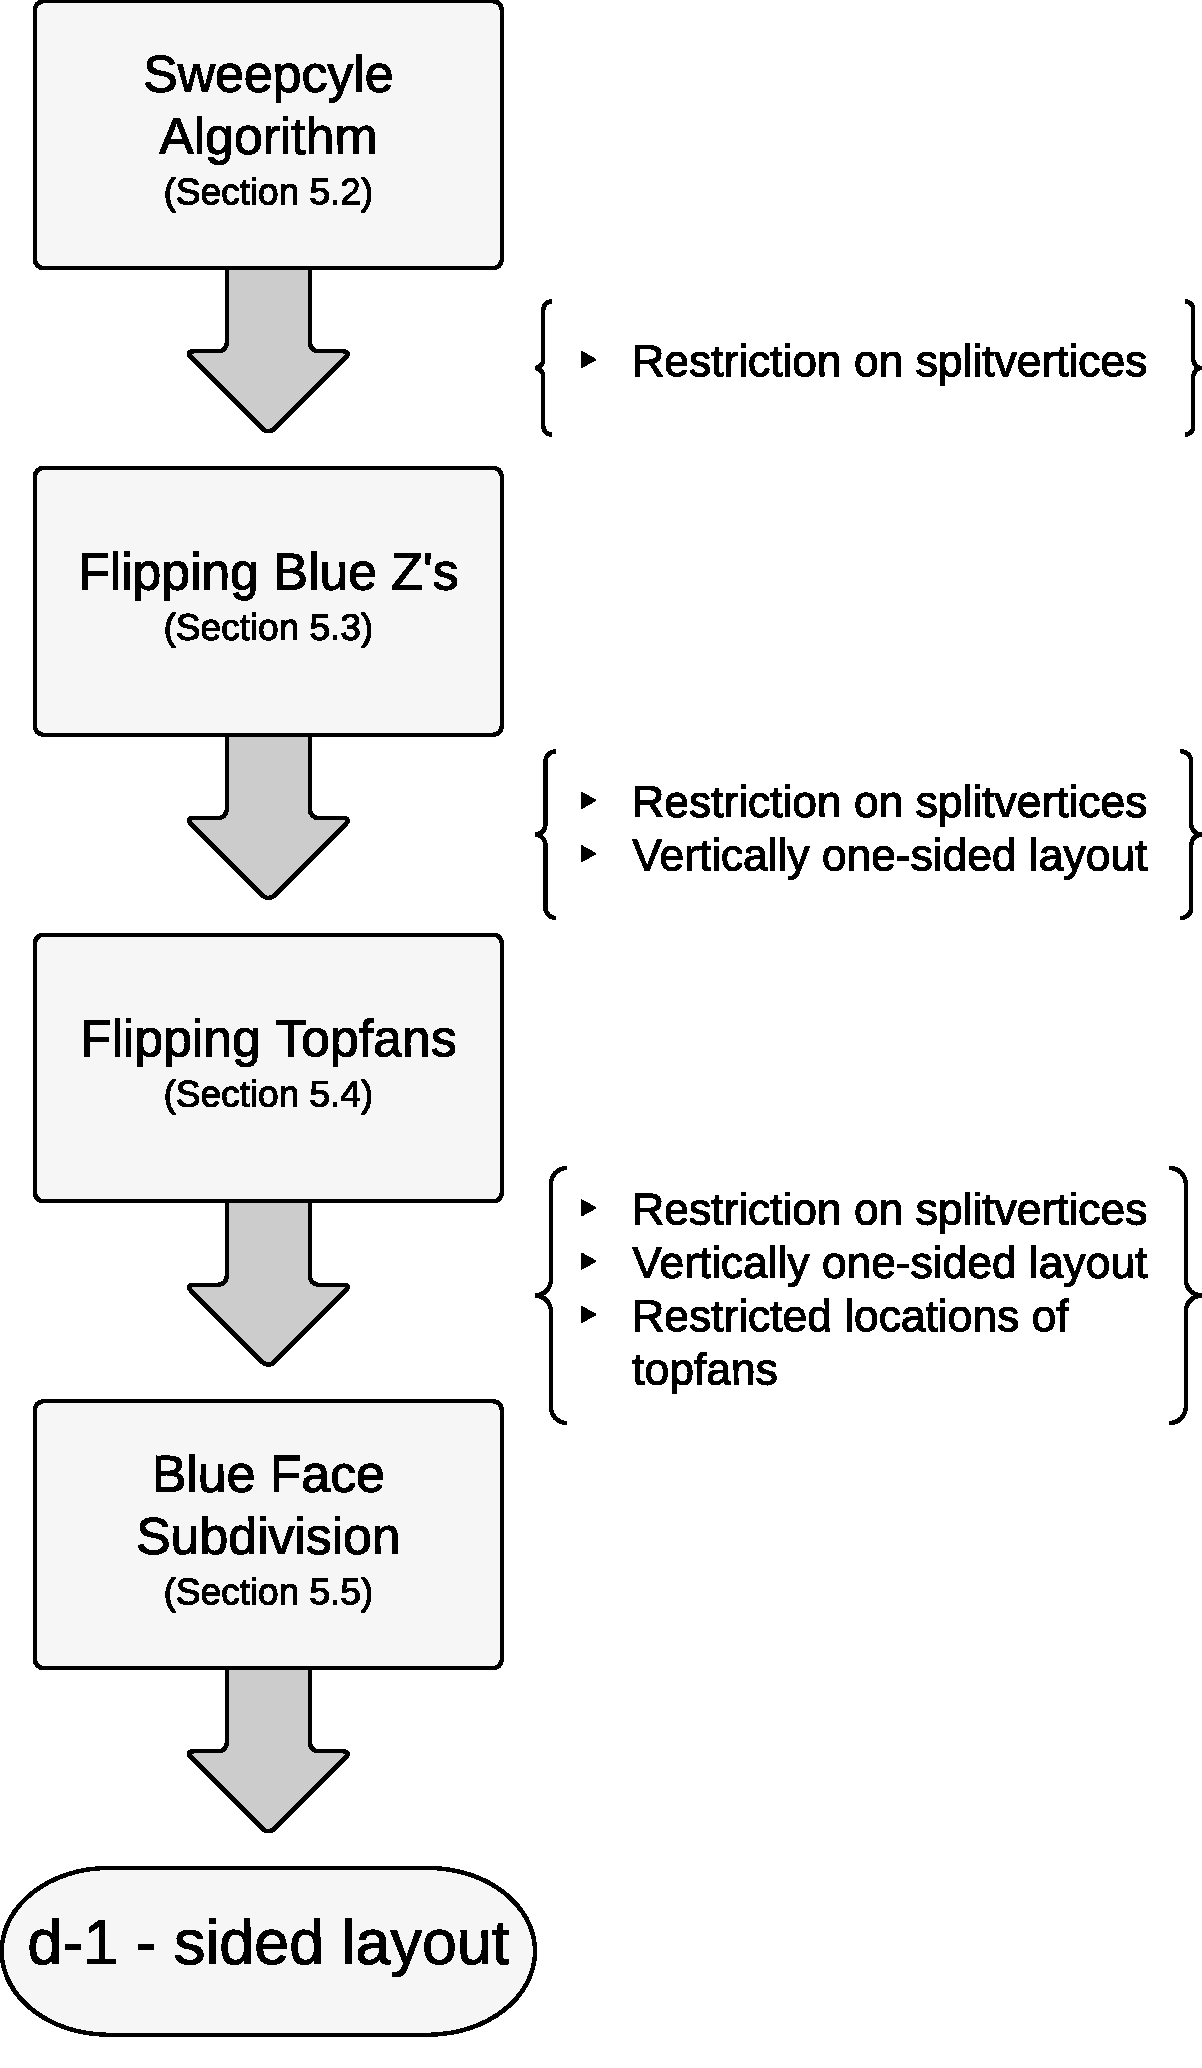
\includegraphics[scale=.37]{unifiedAlgo/img/algoflowext2.pdf}
    \caption{The flow of the algorithm}
    \label{fig:algo:algoflow}
  \end{wrapfigure}

  Our algorithm will need a number of steps to get to the stated result. In Figure~\ref{fig:algo:algoflow} we can see the four main step we need for finding an $d-1$ sided layout. In every step we ensure new restrictions while maintaining the old ones. In the last step, "Blue Face Subdivision", we can than use these accumulated restrictions to build a $d-1$ sided layout.
  \fxnote{Might define topfan to make talking easier}

  The first step is finding a regular edge labeling with a certain restriction on \emph{splitvertices}, vertices having more than one blue outgoing edge.
  We show that these splitvertices can not be next to something we call the handle of a large topfan, that is, a vertex that has more then two incoming red edges.

  In the second step we will make sure that our regular edge labeling $\L$ is \emph{vertically one-sided}. That is, all vertical segments in the corresponding rectangular layout are one-sided segemnts. We can translate this to a condition on the red faces of $\L$, and this condition can then be translated to the existence of a structure we call a \emph{blue $Z$}. In this step we resolve all occurrences of such blue $Z$'s. We suspect that this step is not necessary because the regular edge labeling provided by the sweepcycle algorithm is already vertically one-sided. However, we were unable to proof this.

  The third step then consists of handling most topfans in the regular edge labeling by "Flipping" them. This is the most difficult for those topfans that are adjacent to a splitvertex and hence we have to ignore some of these. If we would have been able to handle all topfans finding a $k$-sided layout would have been easier.

  However, due to the restriction on split vertices we have maintained during the algorithm and the fact that all remaining topfans are adjacent to such splitvertices we are still able to produce an $d-1$ sided layout in the last step.

\fxnote{Is this pargraph still necessary, if yes in what form?}
\mypar{Overview}
  To describe this algorithm we introduce some new concepts in the remainder of this section. Firstly, the notion of right neighbor paths in Section \ref{ss:rightNeighbour}.  We use these right neighbor paths to find a regular edge labeling with some nice properties in Section \ref{ss:sweep}. Afterwards we unfortunately still have to do three post-processing steps. In Section \ref{ss:flipBlueZ} we make sure our regular edge labeling is \emph{vertically one-sided}, that is, that all vertical segments are one-sided. In Section \ref{ss:fanflip} we will remove most occurrences of something called topfans. Then, in Section \ref{ss:subdiv} we can finally subdivide all blue faces that are too large without creating red faces that are too large. This finishes the algorithm.
